%%%%%%%%%%%%%%%%%%%%%%%%%%%%%%%%%%%%%%%%%
% Beamer Presentation
% LaTeX Template
% Version 1.0 (10/11/12)
%
% This template has been downloaded from:
% http://www.LaTeXTemplates.com
%
% License:
% CC BY-NC-SA 3.0 (http://creativecommons.org/licenses/by-nc-sa/3.0/)
%
%%%%%%%%%%%%%%%%%%%%%%%%%%%%%%%%%%%%%%%%%

%----------------------------------------------------------------------------------------
%	PACKAGES AND THEMES
%----------------------------------------------------------------------------------------

\documentclass{beamer}

\mode<presentation> {
	
	% The Beamer class comes with a number of default slide themes
	% which change the colors and layouts of slides. Below this is a list
	% of all the themes, uncomment each in turn to see what they look like.
	
	%\usetheme{default}
	%\usetheme{AnnArbor}
	%\usetheme{Antibes}
	%\usetheme{Bergen}
	%\usetheme{Berkeley}
	%\usetheme{Berlin}
	%\usetheme{Boadilla}
	%\usetheme{CambridgeUS}
	%\usetheme{Copenhagen}
	%\usetheme{Darmstadt}
	%\usetheme{Dresden}
	%\usetheme{Frankfurt}
	%\usetheme{Goettingen}
	%\usetheme{Hannover}
	%\usetheme{Ilmenau}
	%\usetheme{JuanLesPins}
	%\usetheme{Luebeck}
	\usetheme{Madrid}
	%\usetheme{Malmoe}
	%\usetheme{Marburg}
	%\usetheme{Montpellier}
	%\usetheme{PaloAlto}
	%\usetheme{Pittsburgh}
	%\usetheme{Rochester}
	%\usetheme{Singapore}
	%\usetheme{Szeged}
	%\usetheme{Warsaw}
	
	% As well as themes, the Beamer class has a number of color themes
	% for any slide theme. Uncomment each of these in turn to see how it
	% changes the colors of your current slide theme.
	
	%\usecolortheme{albatross}
	%\usecolortheme{beaver}
	%\usecolortheme{beetle}
	%\usecolortheme{crane}
	%\usecolortheme{dolphin}
	%\usecolortheme{dove}
	%\usecolortheme{fly}
	%\usecolortheme{lily}
	%\usecolortheme{orchid}
	%\usecolortheme{rose}
	%\usecolortheme{seagull}
	%\usecolortheme{seahorse}
	%\usecolortheme{whale}
	%\usecolortheme{wolverine}
	
	%\setbeamertemplate{footline} % To remove the footer line in all slides uncomment this line
	%\setbeamertemplate{footline}[page number] % To replace the footer line in all slides with a simple slide count uncomment this line
	
	%\setbeamertemplate{navigation symbols}{} % To remove the navigation symbols from the bottom of all slides uncomment this line
}
\graphicspath{ {images/} }
\usepackage{graphicx} % Allows including images
\usepackage{booktabs} % Allows the use of \toprule, \midrule and \bottomrule in tables
%----------------------------------------------------------------------------------------
%	TITLE PAGE
%----------------------------------------------------------------------------------------

\title[SE Project]{COMP3211 Software Engineering \\
                        Group Project \\
                        Edo - a course management system} % The short title appears at the bottom of every slide, the full title is only on the title page

\author{Fu Kuo-hao 14112466D \\
        Ouyang Xiating 14111773D \\
        Zhou Yi 14109328D} % Your name
\institute % Your institution as it will appear on the bottom of every slide, may be shorthand to save space
{
Department of Computing
}
\date{Dec 1 2016} % Date, can be changed to a custom date

\begin{document}

\begin{frame}
\titlepage % Print the title page as the first slide
\end{frame}

\begin{frame}
\frametitle{Some abbreviations} % Table of contents slide, comment this block out to remove it
\begin{itemize}
	\item Assessment: Assignment and Quiz
	\item Assessment Submission: Assignment and quiz submission
	\item Course content: slides, notes etc.
\end{itemize}
\end{frame}


\begin{frame}
\frametitle{Use Case Diagram}
\begin{figure}[!ht]
	\begin{center}
		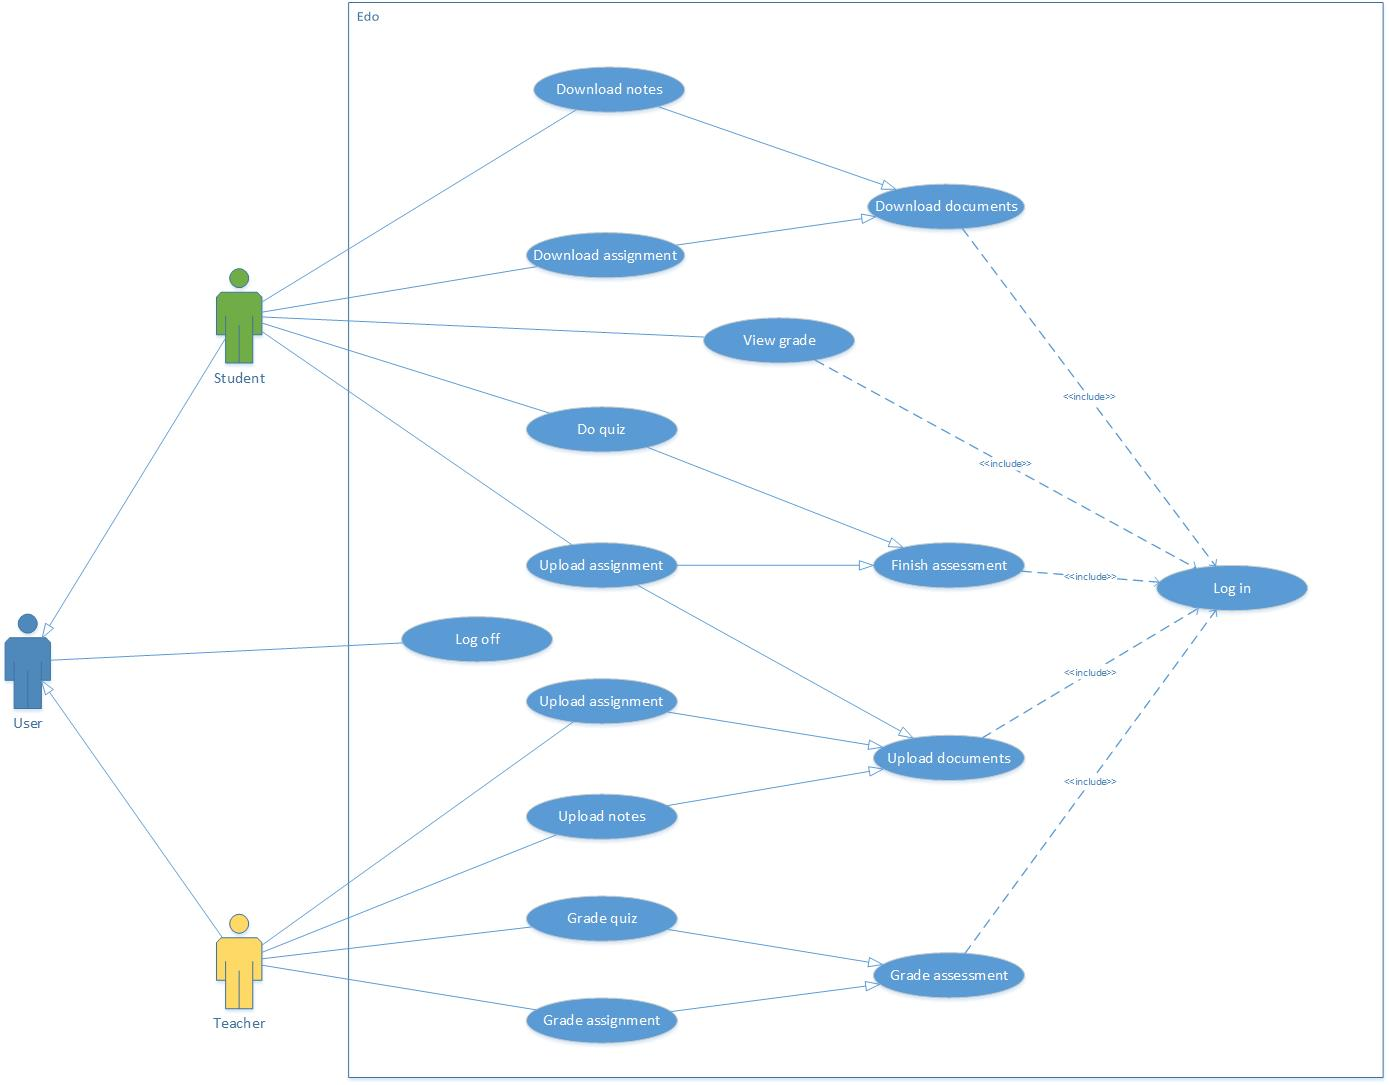
\includegraphics[width=\textwidth,height=0.7\textheight,keepaspectratio]{usecase}
	\end{center}
	\caption{Use Case Diagram}
\end{figure}
\end{frame}

\begin{frame}
	\frametitle{Entity Relationship Diagram}
	\begin{figure}[!ht]
		\begin{center}
			\includegraphics[width=\textwidth,height=0.7\textheight,keepaspectratio]{erd}
		\end{center}
		\caption{ERD}
	\end{figure}
	
\end{frame}



\begin{frame}
	\frametitle{Class Diagram}
	\begin{figure}[!ht]
		\begin{center}
			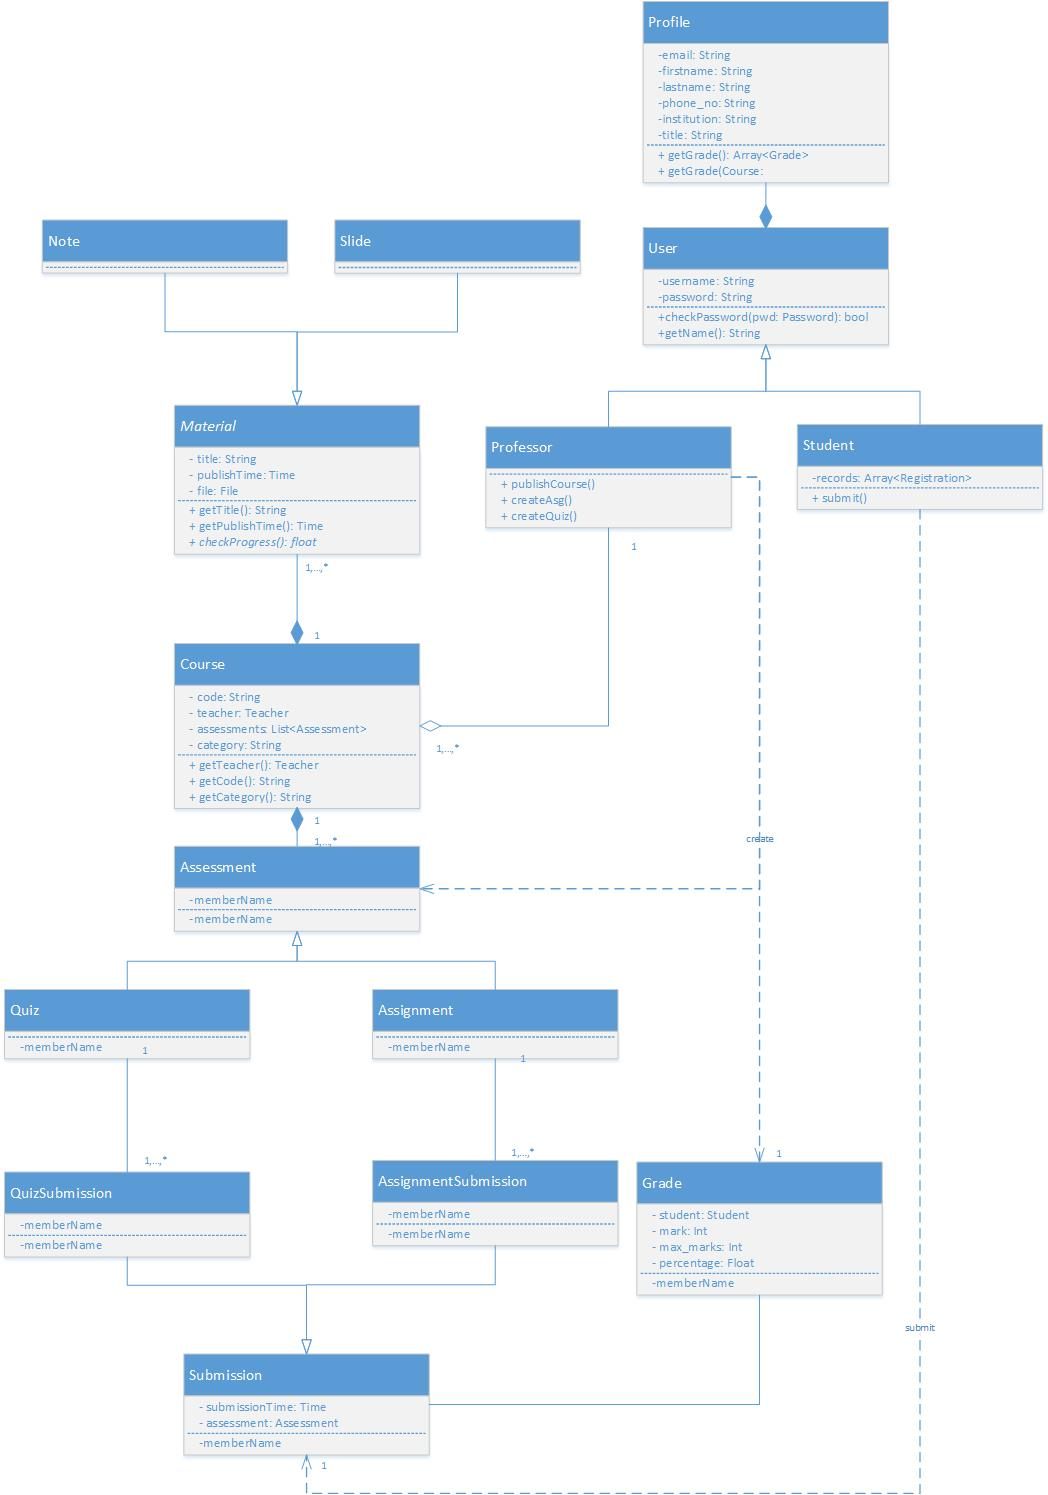
\includegraphics[width=\textwidth,height=0.7\textheight,keepaspectratio]{class}
		\end{center}
		\caption{Class Diagram}
	\end{figure}
	
\end{frame}

\begin{frame}
	\frametitle{System Architectural Diagram}
	\begin{figure}[!ht]
		\begin{center}
			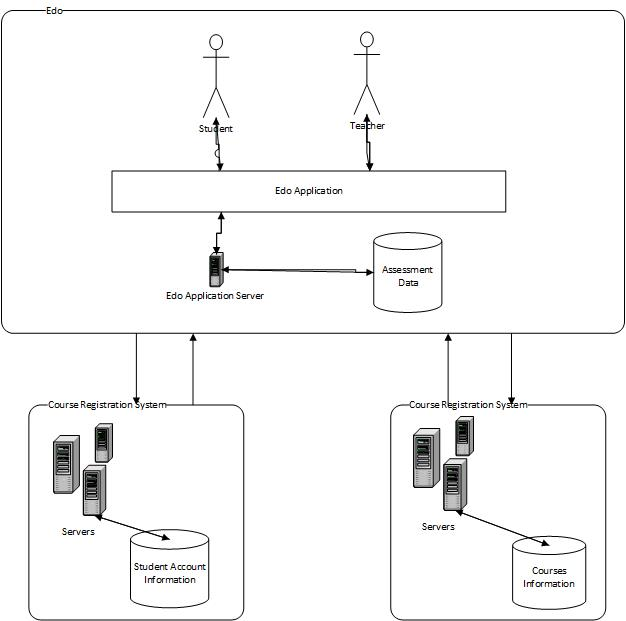
\includegraphics[width=\textwidth,height=0.7\textheight,keepaspectratio]{archi}
		\end{center}
		\caption{Architectural Diagram}
	\end{figure}
	
\end{frame}



\begin{frame}
	\frametitle{State Machine Diagram}
	\begin{figure}[!ht]
		\begin{center}
			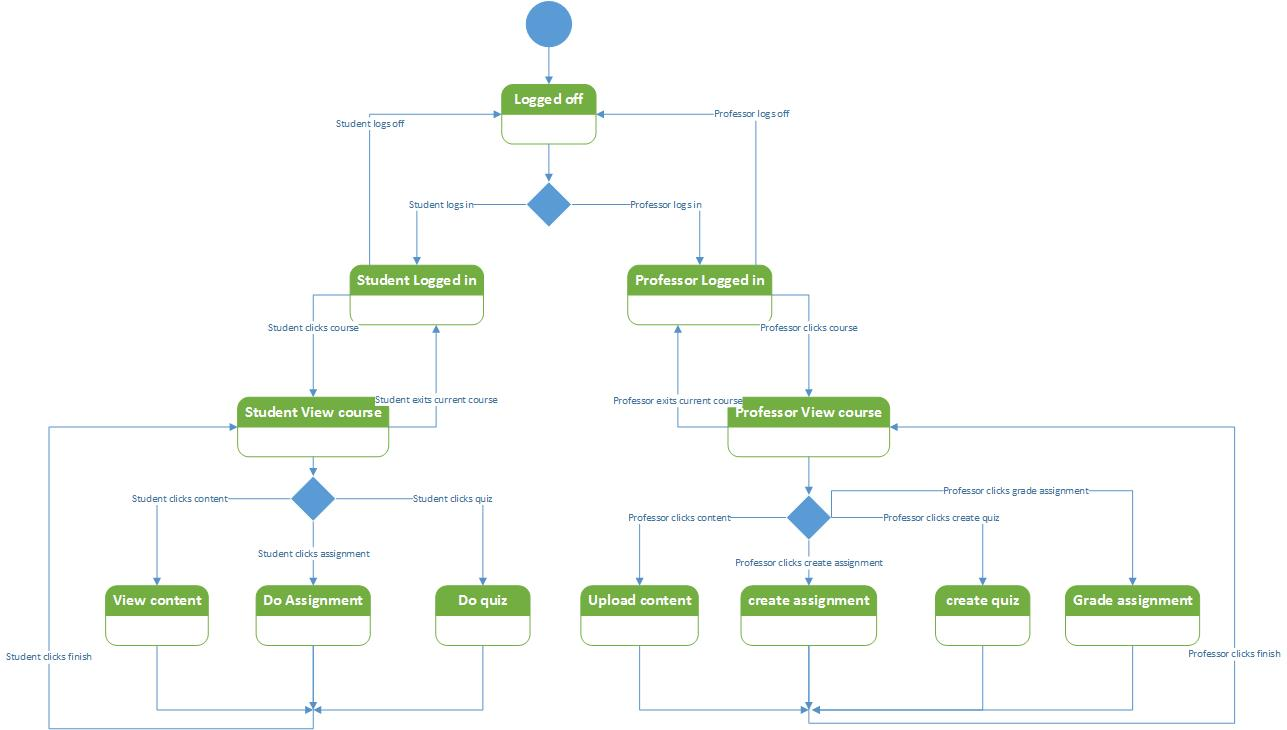
\includegraphics[width=\textwidth,height=0.7\textheight,keepaspectratio]{state}
		\end{center}
		\caption{State Machine Diagram}
	\end{figure}
\end{frame}


\begin{frame}
	\frametitle{Activity Diagram}
	\begin{figure}[!ht]
		\begin{center}
			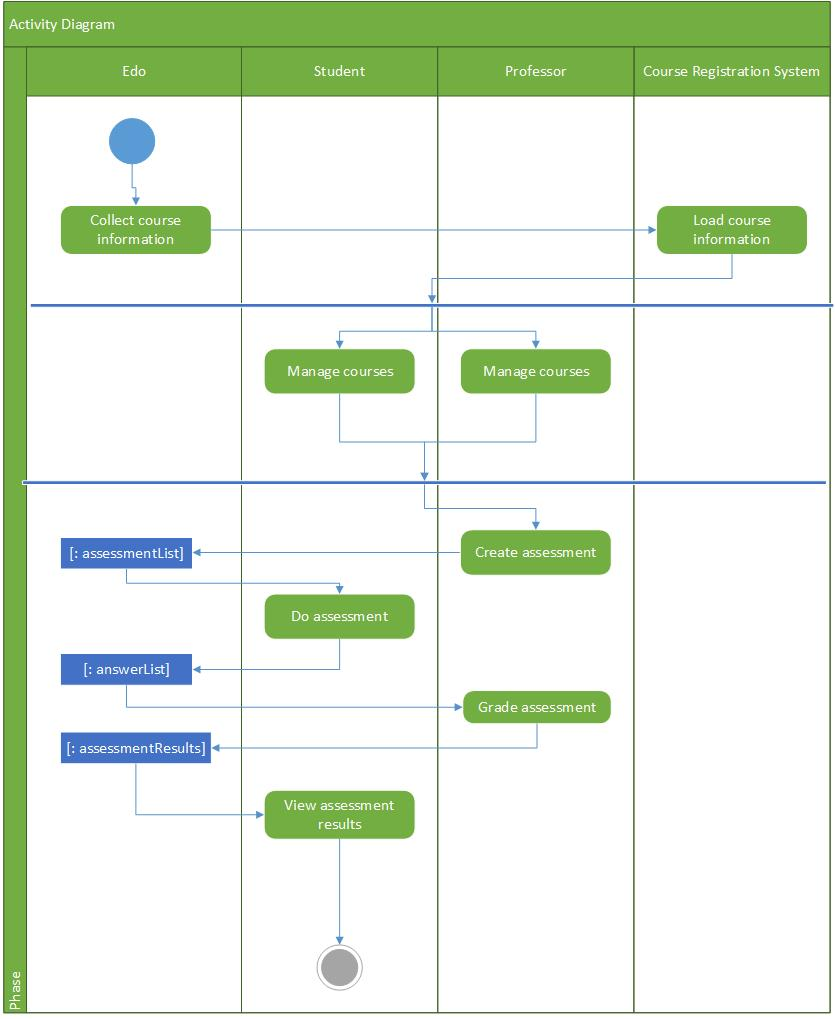
\includegraphics[width=\textwidth,height=0.7\textheight,keepaspectratio]{activity_diagram}
		\end{center}
		\caption{Activity Diagram}
	\end{figure}
	
\end{frame}


\begin{frame}
	\frametitle{Sequence Diagram}
	\begin{figure}[!ht]
		\begin{center}
			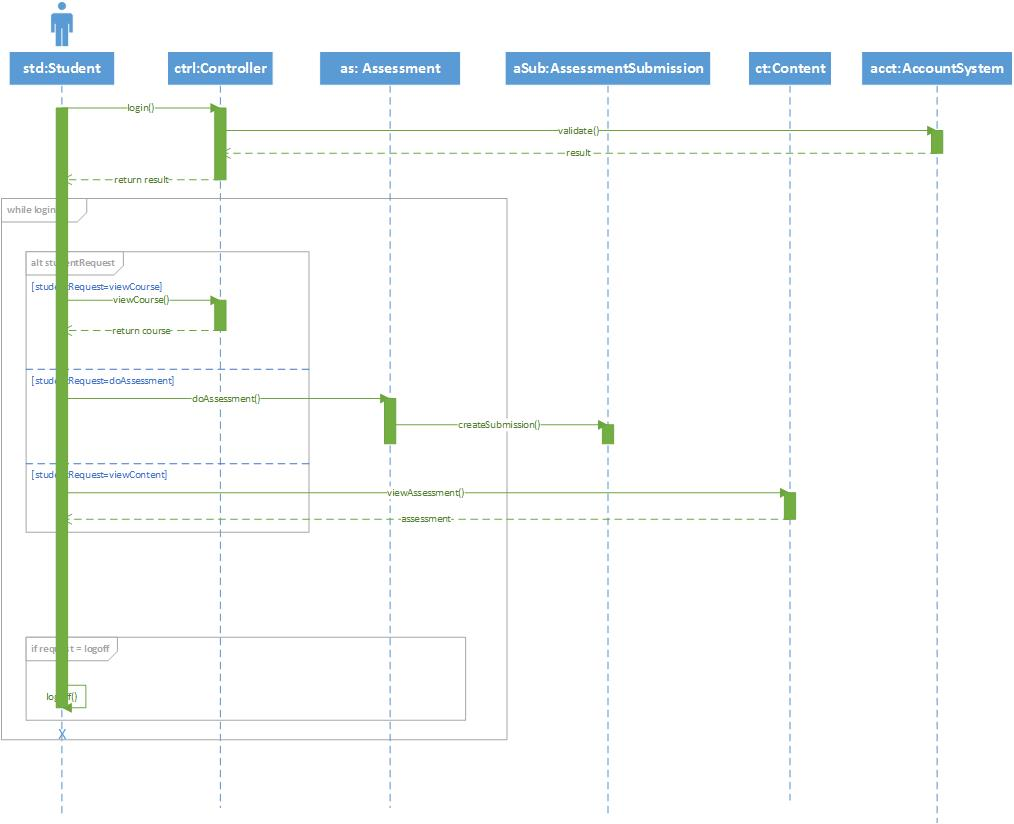
\includegraphics[width=\textwidth,height=0.7\textheight,keepaspectratio]{studSeq}
		\end{center}
		\caption{Sequence Diagram for Students}
	\end{figure}
\end{frame}

\begin{frame}
	\frametitle{Sequence Diagram (cont.)}
	\begin{figure}[!ht]
		\begin{center}
			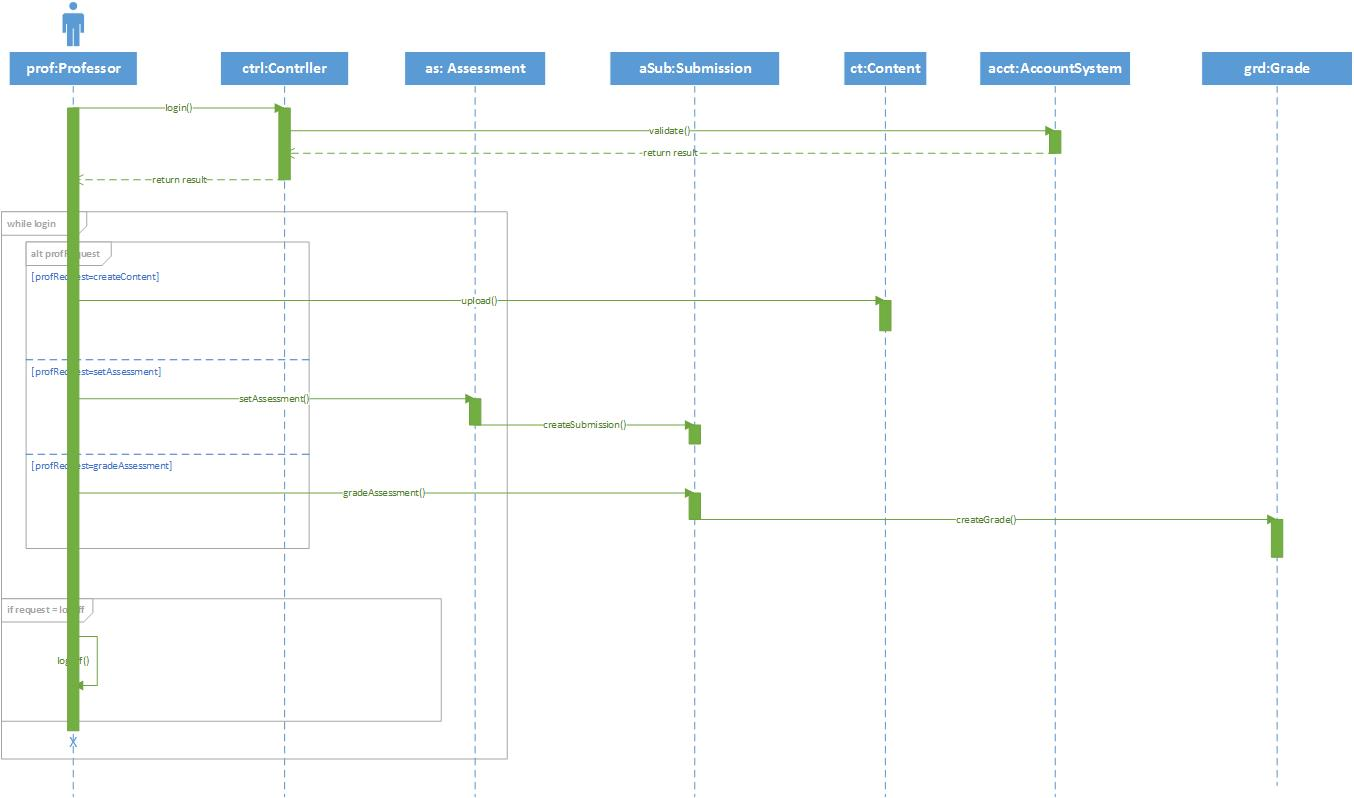
\includegraphics[width=\textwidth,height=0.7\textheight,keepaspectratio]{profSeq}
		\end{center}
		\caption{Sequence Diagram for Professors}
	\end{figure}
\end{frame}

\begin{frame}
\Huge{The End}
\end{frame}

%----------------------------------------------------------------------------------------

\end{document} 